\documentclass[UTF8]{ctexart}

\usepackage{float} 
\usepackage{amsmath}

\title{弹幕游戏的操作序列分析}
\author{卓越羿,郭煌,吴迪}

\begin{document}

\maketitle
\begin{abstract}

摘要内容

\textbf{关键字}: 贝叶斯推断,MCMC,游戏分析


\end{abstract}

\section{问题背景}

游戏正在耗费人类越来越多的时间,所以对于人类在电脑游戏这一形式化的系统上的行为的研究,
无论对于人类自身还是游戏的相关产业都是否有用。
而在对于游戏可能产生的数据,除了在现实中的响应外,最重要的应该是游戏内部的操作序列。
很多游戏可以记录玩家的操作序列,
通常被称为“回放”(replay)。这些回放仅仅包含操作信息,可以重新被游戏读取模拟玩家的操作,以无损失的重现一场游戏的过程。
这与现在流行的通过共享对游戏录制的视频是完全不同的,视频不用具有游戏即可以播放,但仅能记录画面的信息,
而这些画面信息完全可以由大小小多了的操作序列通过运行游戏重造出来。早期网络的网速较慢,
出于与现在视频流行类似的共享需求,回放技术得到了发展。

电脑游戏回放中可能最多的,是即时战略游戏的回放,虽然存在一些相关的分析
%(此处应有对kaggle那个星际争霸回放研究的引用,以及引用的引用),
\cite{starcraft}
但是这些信息比较复杂,
我们可以对比另外也许是“回放”很多的非电脑游戏,如国际象棋和围棋,可以以“棋谱”为形式记录它们,
有着它们行为空间固有的简单性。只需注意到这些游戏上的人工智能取得成就
%(此处引用alphago),
\cite{alphago}
就可以意识到这一点。对于类似的输入简单地游戏,
如那些游戏机上只通过手柄的有限的按键输入的游戏,人工智能也取得了类似的成就,
如有名的DQN算法
%(引用Atari游戏论文),
\cite{atari}
其必须基于输入的离散性。
我们这里也研究一种类似的游戏,即弹幕游戏(STG)。

弹幕游戏主要是玩家在操纵角色躲避敌方“弹幕”同时进行反击的游戏,
其挑战性主要在于玩家的反应速度与根据弹幕运动规律进行预判(被称为“底力”),
在更深度的玩家那里,记忆特定关卡的弹幕特征也是重要的(称为“背板”)。有名的弹幕游戏系列包括雷电,虫姬等,
我们这里研究玩家较多,从而积累下的回放数也较多的东方project系列,其中的第10部,风神录作为具体研究的游戏。

游戏的回放文件批量下载自回放存档网站royalflare\footnote{ http://score.royalflare.net/ }。
该网站保存了过往玩家自发上传的回放,通常属于打出彩的那种。
我们主要选择其中Lunatic难度(最高难度)“梦B型”的202个回放文件,其跨度从2007到2017年。

\section{原始数据类型与数据处理}

回放文件是二进制的,其包含元信息-关卡信息,关卡信息又包含关卡的元信息与该关卡的操作序列,
操作序列是整个回放文件的主要数据。

操作序列由一系列48bit的数据块构成,其表示一帧(frame,通常来说1秒=60frame)中的按键情况。
我们大致的实验揭示了以下部分重要按键与数据的关系:

\begin{verbatim}
000000000000000000000000000100000000000000000000
                       ***** ***                 
*标出的二进制位分别表示 这帧正在按着 ctrl, right, left, down, up, shift,x,z
000000000001000000000000000101000000000000000000
       ***** ***                                
*标出的二进制位分别表示 这帧刚刚按下了 ctrl, right, left, down, up, shift,x,z
000000000000000000000000000000000000000111110111
                                       ***** ***
*标出的二进制位分别表示 这帧 刚刚松开 ctrl, right,left,down,up,shift,x,z
\end{verbatim}
                                       
如上文所示,第一个数据块那个1表示该帧中玩家正在按up(方向键向上)键,
第二个数据则表示该帧玩家刚按下了up,且从之前开始就按着shift。

48bit的数据块可以看做48个01变量,这里展示了24个键位的含义,
分别为表示当前帧按下,按中,松开ctrl,右,左,下,上,shift,x,z键。
其他键可能表示Esc和一些特殊按键的三种情况,不过未做实验。

为了解析这些二进制文件,我们编写了Python程序并传到GitHub上 
\footnote{ https://github.com/yiyuezhuo/touhou-replay-decoder }
但其中一些具体的解析的“魔数”的提供是由  threp \footnote{ https://github.com/Fluorohydride/threp } 进行的,
不幸的是其中有一些bug而原始实现的C语言不好调试,所以我们实现了Python版并强化了API。

上述程序的一个功能是将二进制文件转成json文件,这也是我们将作为附件的内容。
但代码里主要使用Python的pickle暂存的文件。
因为数据占用内存太多对后面的贝叶斯推断程序无法执行。解码程序本身可在上面的github页面查到,
转换程序在explore\_help.py中。

虽然做过全部数据的探索,但下面我们只会提到这样的数据,202个回放现在每一个对应6个关卡(stage)的秒序列,
每秒对应一个四个变量的记录,表示这秒60帧中按下shift,ctrl,x按键的帧数,与“绝对运动量”,
即按下一秒内按下四个方向键的帧数和。

其中shift是慢速移动的键,按下这键表示当前的场景比较紧张,需要精细移动。ctrl是跳过对话的键,
表明了此时处于特定的对话阶段。x是“灵击”,表明此时是刷分时刻或危险时刻。
绝对移动量是根据是否当前帧处于慢速移动还是正常移动,在上下左右按键情况加权下的指标。具体来说,该秒内
某帧按住shift时还按下“下”(此时也可以按其他键,类似计算),将在该指数中+2.0,若没有按下shift则加4.5,
若并没有按下“下”则贡献0。虽然计算了互相1s内相互抵消的相对移动量,但没有纳入分析。

\section{探索式分析}

\subsection{轨迹图}

根据东方系列wiki所述\footnote{ http://wikiwiki.jp/thk/?\%C9\%F7\%2FPlayer } 在按着shift时的移动,
即慢速移动,在我们考虑的“梦B”类中为 2像素/秒。而不按着shift时的移动,即快速移动速度为 4.5像素/秒。
故按照这个情况可以绘制一关内玩家控制的机体的移动轨迹,这对于确认二进制分析是否正确也是重要的。

\begin{figure}[H]
\begin{minipage}[t]{0.5\linewidth}
\centering
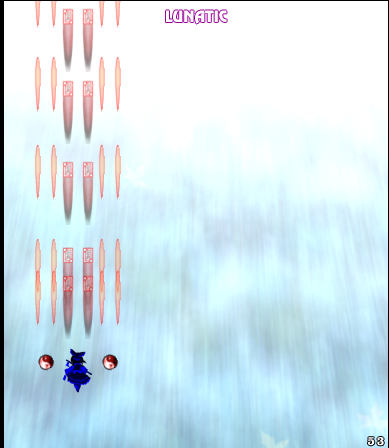
\includegraphics[width=2.2in]{images/touhou1.png}
\caption{时刻1}
\end{minipage}%
\begin{minipage}[t]{0.5\linewidth}
\centering
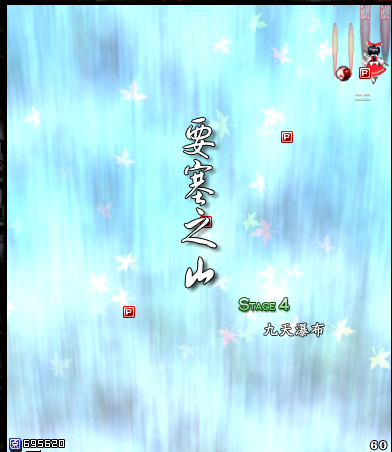
\includegraphics[width=2.2in]{images/touhou2.png}
\caption{时刻2}
\end{minipage}
\begin{minipage}[t]{0.5\linewidth}
\centering
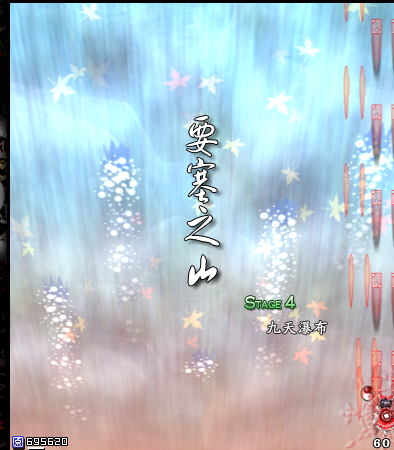
\includegraphics[width=2.2in]{images/touhou3.png}
\caption{时刻3}
\end{minipage}
\begin{minipage}[t]{0.5\linewidth}
\centering
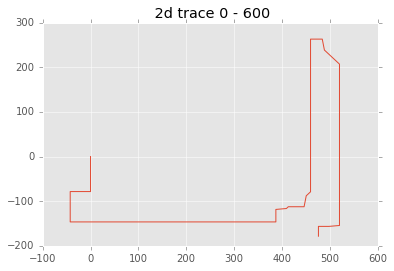
\includegraphics[width=2.2in]{images/trace2d.png}
\caption{2d轨迹图}
\end{minipage}
\begin{minipage}[t]{0.5\linewidth}
\centering
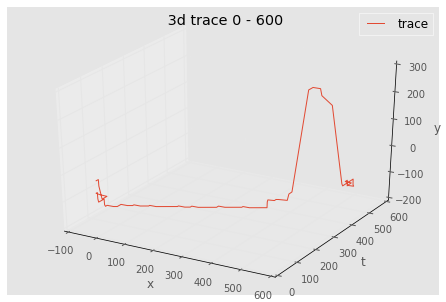
\includegraphics[width=2.2in]{images/trace3d.png}
\caption{3d轨迹图}
\end{minipage}
\begin{minipage}[t]{0.5\linewidth}
\centering
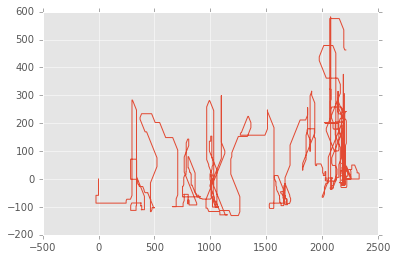
\includegraphics[width=2.2in]{images/trace2dfull.png}
\caption{该时间段完整2d轨迹图}
\end{minipage}
\end{figure}

上图1,2,3展示了某个回放在第四关开头的三个瞬间,而我们对存档解析出的2d轨迹图各帧的移动轨迹。
考虑到在同一轨迹上移动或停止与速度变化并不能体现在2d轨迹图上,我们还绘制了3d轨迹图。
最后一张图展示了该关整个轨迹。由于玩家控制的自机被摧毁时会重置位置,这个连续的轨迹图并不能反映除了开始一段时间外
的位置情况(但通过取其中一些点将部分轨迹平移可以做到,这里并没有展示。)

\begin{figure}[H]
\begin{minipage}[t]{0.5\linewidth}
\centering
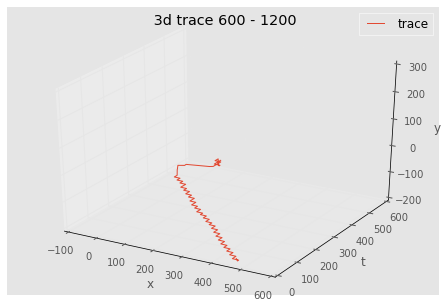
\includegraphics[width=2.2in]{images/trace3dsm.png}
\caption{微移移动行为}
\end{minipage}%
\begin{minipage}[t]{0.5\linewidth}
\centering
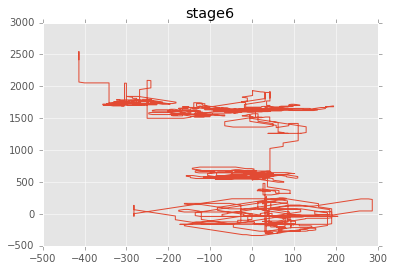
\includegraphics[width=2.2in]{images/trace2dstage6.png}
\caption{时刻2}
\end{minipage}
\end{figure}

而从左图是上图那个600帧后的600帧的3d轨迹图中,我们可以从中看到锯齿型(这在2d图中则难以看出,就是一个横线)
看出该类游戏的一个典型行为,即通过“微移”来躲避所谓的“自机狙”,锯齿的产生是因为按一下左键马上松开再按这种行为,
这种行为可以在按住shift的基础上进一步降低平均速度,故而称为“微移”行为。

右图是同一个回放第六关的完全轨迹图,虽然并不能把其当做位置轨迹,
但可以明显的看到很多时间内玩家被困在一块小区域里运动的模式。这与这关的敌人的封锁能力有关。

\subsection{按键情况时序图}

\begin{figure}[H]
\begin{minipage}[t]{0.5\linewidth}
\centering
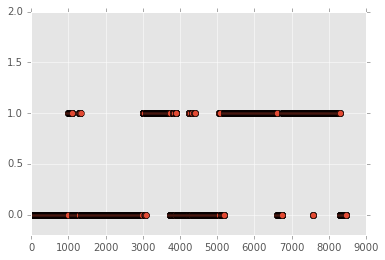
\includegraphics[width=2.2in]{images/pressingShiftFrame.png}
\caption{按帧计的按下shift的0,1序列}
\end{minipage}%
\begin{minipage}[t]{0.5\linewidth}
\centering
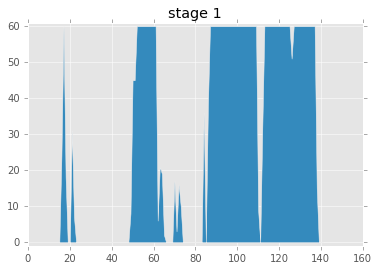
\includegraphics[width=2.2in]{images/pressingShift1.png}
\caption{按秒求和的}
\end{minipage}
\end{figure}

如果直接显示当前帧正在按住shift的0,1时序图。将是左图的样子,这样显然很难看出更细致的东西,而按1秒=60帧
\footnote{严格来说,这与玩家真正的秒不一定一致,此指标即所谓的fps,帧每秒。
游戏至多把fps可能升到60以上的时候控制在60,却不能在其低于60的时候将其无损失的提升到60。
不过本文就称60帧为1秒为了方便 }求和后。图就变成了右边那样,显然更加清晰。

前文指出过按住shift表示当时的局势比较紧张,所以可以从按住shift的情况中分辨出各个关卡的特征。
正如下面同一个回放中六个关卡的按秒求和的时序图所示:

\begin{figure}[H]
\begin{minipage}[t]{0.5\linewidth}
\centering
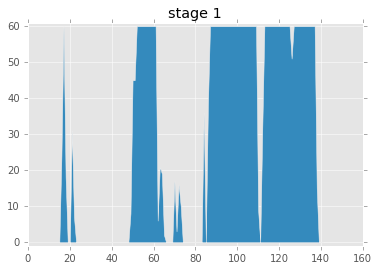
\includegraphics[width=2.2in]{images/pressingShift1.png}
\end{minipage}
\begin{minipage}[t]{0.5\linewidth}
\centering
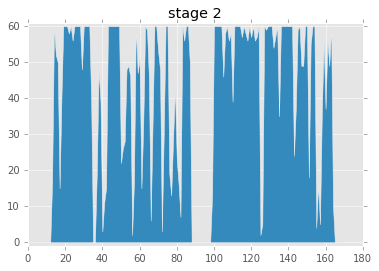
\includegraphics[width=2.2in]{images/pressingShift2.png}
\end{minipage}
\begin{minipage}[t]{0.5\linewidth}
\centering
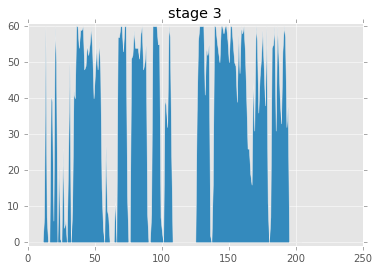
\includegraphics[width=2.2in]{images/pressingShift3.png}
\end{minipage}
\begin{minipage}[t]{0.5\linewidth}
\centering
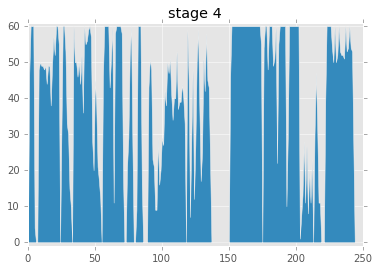
\includegraphics[width=2.2in]{images/pressingShift4.png}
\end{minipage}
\begin{minipage}[t]{0.5\linewidth}
\centering
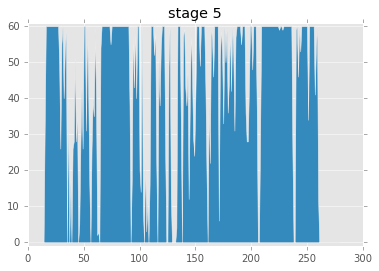
\includegraphics[width=2.2in]{images/pressingShift5.png}
\end{minipage}
\begin{minipage}[t]{0.5\linewidth}
\centering
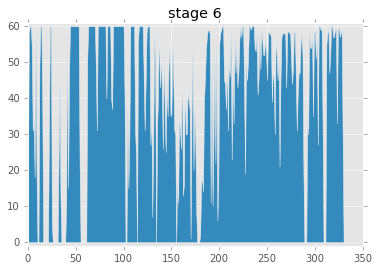
\includegraphics[width=2.2in]{images/pressingShift6.png}
\end{minipage}
\end{figure}

尽管其他按键的时序图也是有趣的,但这里略去,部分信息可以由下面的图反映出来。

\subsection{按时间在各回放上直接求和}

东方的一个关卡分为若干阶段,有的阶段时间固定,有的不固定,有的还根据之前的情况出现或不出现。
玩家则根据策略不同,会选择不同的打法,如“刷分”打法可能会使时间可变的阶段尽可能持续的更久,
而“混关”打法则可能倾向于快速通过以回避遭到损失的不确定性。这一策略的混合下在下图中展示的非常清楚:

\begin{figure}[H]
\centering
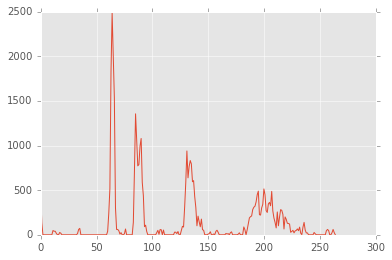
\includegraphics[width=\linewidth]{images/pressingCtrlSum.png}
\caption{在202个回放上在第三关上以按住ctrl帧数求和}
\end{figure}

202个回放在第三关各秒,直接对按住ctrl求和的结果。按住ctrl通常是为了跳过对话,而对话在某些固定阶段过渡时发生,
于是上述峰可以用于划分阶段。而峰的分布反映了混合策略存在的可能性,显然,
如果所有回放中玩家的策略和实施情况一样,则峰应该重叠在一秒上。而这并没有发生,

峰越来越的矮胖除了可以看做独立同分布的间隔叠加的结果外,和后面阶段本身的玩家可控制的时间范围也有关。
而若要仔细识别个别玩家使用的策略或者统计的推论可能策略数,必须借助后面的统计模型。

为了展示ctrl划分的阶段并不是按住ctrl变量内部独有的现象,下面我们在上图基础上画出按住x的情况进行对比:

\begin{figure}[H]
\begin{minipage}[t]{0.5\linewidth}
\centering
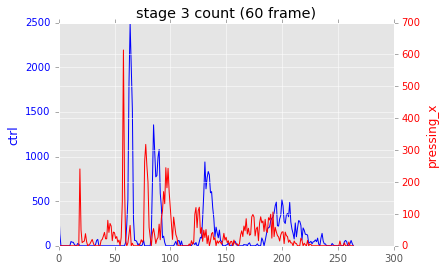
\includegraphics[width=2.2in]{images/sumCtrlX.png}
\caption{第三关ctrl与X按键}
\end{minipage}%
\begin{minipage}[t]{0.5\linewidth}
\centering
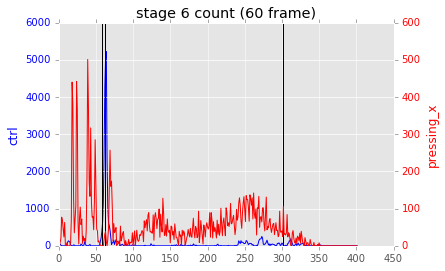
\includegraphics[width=2.2in]{images/sumCtrlX2.png}
\caption{第六关ctrl与X按键}
\end{minipage}
\end{figure}

如果左图还不明显,我们可以在反映第六关相同关系的右图中明显发现在黑线标出的估计的分界点过后,
x的按键情况也发生了很大变化。所以ctrl是指示阶段变化的很好的变量。

\section{统计分析}

探索式分析提供的信息可以被进一步的精确统计分析更好的分析。

\subsection{分界点问题}



\subsubsection{模型设定}

符号约定:

下面均指在一个特定关卡内,由于内存限制没有做跨关卡的分析

\begin{tabular}{c|c}
 \hline
 $N$ & 回放总数 \\
 $P$ & 阶段数 \\
 $Sh_{it}$ & 第$i$个回放在第$t$秒的按住Shift的帧数 \\
 $Ct_{it}$ & 第$i$个回放在第$t$秒的按住Ctrl的帧数 \\
 $X_{it}$ & 第$i$个回放在第$t$秒的按住X的帧数 \\
 $move_{it}$ & 第$i$个回放在第$t$秒的绝对移动量 \\
 $d_{ip}$ & 第$i$个回放在第$p$阶段的持续秒数 \\
 $b_{ip}$ & 第$i$个回放$p$阶段的结束时间 \\
 $p_{it}$ & 第$i$个回放在第$t$秒处于的阶段 \\
\end{tabular}

对联合概率的分层描述:

\begin{align*} % *是去掉公式编号。。上次就被这个坑了
& d_{ip} \sim N(\mu^d_i,\sigma^d_i) \quad i = 1,\dots,N \quad p = 1,\dots,P \\
& b_{ip} = \sum_{h=1}^p d_{ih} \\
& p_{it} = \max( \{ p \mid t < b_{ip} \quad p = 1,\dots,P \} ) \\
& \mu^{Sh}_p \sim Exp(1/\bar{\mu^{Sh}_p}) \quad p = 1,\dots,P \\
& \mu^{Ct}_p \sim Exp(1/\bar{\mu^{Ct}_p}) \\
& \mu^{X}_p \sim Exp(1/\bar{\mu^{X}_p}) \\
& \mu^{move}_p \sim Exp(1/\bar{\mu^{move}_p}) \\
& \sigma^{move}_p \sim Exp(1/\bar{\sigma^{move}_p}) \\
& Sh_{it} \sim Poi(\mu^{Sh}_{p_{it}}) \\
& Ct_{it} \sim Poi(\mu^{Ct}_{p_{it}}) \\
& X_{it} \sim Poi(\mu^{X}_{p_{it}}) \\
& move_{it} \sim N(\mu^{move}_{p_{it}},\sigma^{move}_{p_{it}}) \\
\end{align*}

这里$\bar{\mu}^{Y}_{p}$,($Y$可能为$Sh,Ct,X,move,d$等)为给定的参数。
控制了随机参数$\mu^{Y}_p$的先验分布。它们采用指数分布是为了连续且保持正数性。
$Sh_{ti},Ct_{it},X_{it}$服从泊松分布是因为取值为整数。

该模型指定的四个变量$Sh,Ct,X,move$在给定其所在状态$p_{it}$下互相条件独立,同时在$i,t$内部上也独立。

该模型的可观测变量是$Sh_{it},Ct_{it},X_{it},move_{it}$。
重要的潜在变量是$d_{ip}$,显然阶段内的四个变量的共性将同时为阶段持续时间
或者说分割点提供信息,这应该比平凡的,如之前展示的根据ctrl计算的估计的分割点更强。


\subsubsection{推断}


为了增加运行效率和编写模型方便,使用了Edward,一个用来概率编程的Python库\cite{edward}。
由于模型的复杂性,为了求解给定数据的隐变量分布与随机参数的后验分布,必须借助近似方法。
流行的近似后验分布的方法有MCMC(马尔科夫链蒙特卡洛法)和变分推断,这里本来是打算采用经典的Metropolis-Hastings算法,
\cite{metropolis}
但一次抽样全部维度接受率太低,加上一次采样本来就要消耗很多内存,为了尽可能采集到有效地样本,
换用部分的Gibbs采样\cite{gibbs},Edward或PyMC3之类的概率编程框架由于基于tensorflow或theano这些构建计算图的框架,
所以真正的ElementWise的Gibbs采样开销太高,故而它们都没有提供真正的Gibbs采样法。
我们自己实现了一个在几个向量之间轮换采样的算法,可以说介于MH与Gibbs之间,但内存开销已经处于无法使用的临界点中。


\subsection{策略识别}

%参考文献
\begin{thebibliography}{9}%宽度9
 \bibitem{alphago} Silver D, Huang A, Maddison C J, et al. Mastering the game of Go with deep neural networks and tree search[J]. Nature, 2016, 529(7587): 484-489. 	
 \bibitem{starcraft} Hostetler J, Dereszynski E W, Dietterich T G, et al. Inferring strategies from limited reconnaissance in real-time strategy games[J]. arXiv preprint arXiv:1210.4880, 2012.
 \bibitem{atari} Mnih V, Kavukcuoglu K, Silver D, et al. Playing atari with deep reinforcement learning[J]. arXiv preprint arXiv:1312.5602, 2013.
 \bibitem{edward} Tran D, Kucukelbir A, Dieng A B, et al. Edward: A library for probabilistic modeling, inference, and criticism[J]. arXiv preprint arXiv:1610.09787, 2016.
 \bibitem{metropolis} Hastings W K. Monte Carlo sampling methods using Markov chains and their applications[J]. Biometrika, 1970, 57(1): 97-109..
 \bibitem{gibbs} Geman S, Geman D. Stochastic relaxation, Gibbs distributions, and the Bayesian restoration of images[J]. IEEE Transactions on pattern analysis and machine intelligence, 1984 (6): 721-741.
\end{thebibliography}

\newpage
%附录
\appendix
附录内容


\end{document}